\documentclass[11pt]{article}
\usepackage[utf8]{inputenc}

\usepackage{latexsym}
\usepackage{amssymb,amsmath}
\usepackage{graphicx}
\usepackage{sgame}
\usepackage{color}
\usepackage{authblk}

% \usepackage{hyperref}
\usepackage{empheq}
\usepackage{blkarray}
\usepackage{cancel}
\usepackage{enumerate}
\usepackage{times}
\usepackage{array}
\usepackage{lscape}

\usepackage[margin=.75in]{geometry}
\newcommand{\newword}[1]{\textbf{\emph{#1}}}

%Arrows
\newcommand{\into}{\hookrightarrow}
\newcommand{\onto}{\twoheadrightarrow}

%Macros
\newcommand{\isom}{\cong} %The isomorphism symbol
\newcommand{\union}{\cup}
\newcommand{\intersection}{\cap}
\newcommand{\bigunion}{\bigcup}
\newcommand{\bigintersection}{\bigcap}
\newcommand{\disjointunion}{\sqcup}
\newcommand{\bigdisjointunion}{\bigsqcup}

\newcommand\numberthis{\addtocounter{equation}{1}\tag{\theequation}}

%Some multiletter functions
\DeclareMathOperator{\Hom}{Hom}
\DeclareMathOperator{\Ext}{Ext}
\DeclareMathOperator{\End}{End}
\DeclareMathOperator{\Tor}{Tor}
\DeclareMathOperator{\Ker}{Ker}
\DeclareMathOperator{\CoKer}{CoKer}
\DeclareMathOperator{\Spec}{Spec}
\DeclareMathOperator{\Proj}{Proj}
\renewcommand{\Im}{\mathop{\mathrm{Im}}}
%Their calligraphic versions; use these for the sheaf constructions
\DeclareMathOperator{\HHom}{\mathcal{H} \textit{om}}
\DeclareMathOperator{\EExt}{\mathcal{E} \textit{xt}}
\DeclareMathOperator{\EEnd}{\mathcal{E} \textit{nd}}
\DeclareMathOperator{\TTor}{\mathcal{T} \textit{or}}
\DeclareMathOperator{\KKer}{\mathcal{K}\textit{er}}
\DeclareMathOperator{\CCoKer}{\mathcal{C} \textit{o}\mathcal{K} \textit{er}}
\newcommand{\IIm}{\mathop{\mathcal{I} \textit{m}}}
\newcommand{\ccH}{\mathscr{H}} %The very curly H

\DeclareMathOperator{\sss}{\mathrm{sunny}}
\DeclareMathOperator{\rrr}{\mathrm{rainy}}
\DeclareMathOperator{\hhh}{\mathrm{hot}}
\DeclareMathOperator{\ccc}{\mathrm{cold}}


%This makes alternating tensors look right in displayed equations
\newcommand{\Alt}{\bigwedge\nolimits}

%Blackboard bold letters

\renewcommand{\AA}{\mathbb{A}}
\newcommand{\BB}{\mathbb{B}}
\newcommand{\CC}{\mathbb{C}}
\newcommand{\DD}{\mathbb{D}}
\newcommand{\EE}{\mathbb{E}}
\newcommand{\FF}{\mathbb{F}}
\newcommand{\GG}{\mathbb{G}}
\newcommand{\HH}{\mathbb{H}}
\newcommand{\II}{\mathbb{I}}
\newcommand{\JJ}{\mathbb{J}}
\newcommand{\KK}{\mathbb{K}}
\newcommand{\LL}{\mathbb{L}}
\newcommand{\MM}{\mathbb{M}}
\newcommand{\NN}{\mathbb{N}}
\newcommand{\OO}{\mathbb{O}}
\newcommand{\PP}{\mathbb{P}}
\newcommand{\QQ}{\mathbb{Q}}
\newcommand{\RR}{\mathbb{R}}
\renewcommand{\SS}{\mathbb{S}}
\newcommand{\TT}{\mathbb{T}}
\newcommand{\UU}{\mathbb{U}}
\newcommand{\VV}{\mathbb{V}}
\newcommand{\WW}{\mathbb{W}}
\newcommand{\XX}{\mathbb{X}}
\newcommand{\YY}{\mathbb{Y}}
\newcommand{\ZZ}{\mathbb{Z}}

%Calligraphic letters

\newcommand{\cA}{\mathcal{A}}
\newcommand{\cB}{\mathcal{B}}
\newcommand{\cC}{\mathcal{C}}
\newcommand{\cD}{\mathcal{D}}
\newcommand{\cE}{\mathcal{E}}
\newcommand{\cF}{\mathcal{F}}
\newcommand{\cG}{\mathcal{G}}
\newcommand{\cH}{\mathcal{H}}
\newcommand{\cI}{\mathcal{I}}
\newcommand{\cJ}{\mathcal{J}}
\newcommand{\cK}{\mathcal{K}}
\newcommand{\cL}{\mathcal{L}}
\newcommand{\cM}{\mathcal{M}}
\newcommand{\cN}{\mathcal{N}}
\newcommand{\cO}{\mathcal{O}}
\newcommand{\cP}{\mathcal{P}}
\newcommand{\cQ}{\mathcal{Q}}
\newcommand{\cR}{\mathcal{R}}
\newcommand{\cS}{\mathcal{S}}
\newcommand{\cT}{\mathcal{T}}
\newcommand{\cU}{\mathcal{U}}
\newcommand{\cV}{\mathcal{V}}
\newcommand{\cW}{\mathcal{W}}
\newcommand{\cX}{\mathcal{X}}
\newcommand{\cY}{\mathcal{Y}}
\newcommand{\cZ}{\mathcal{Z}}


\DeclareMathOperator{\ord}{ord}
\DeclareMathOperator{\inte}{int}
\DeclareMathOperator{\nhd}{nhd}

\newcommand{\ds}{\displaystyle}
\newcommand{\mc}{\mathcal}
\newcommand{\ol}{\overline}
\newcommand{\modu}{\hspace{-2mm} \mod}

\DeclareMathOperator{\inn}{Inn}
\DeclareMathOperator{\aut}{Aut}
\DeclareMathOperator{\cen}{Center}
\DeclareMathOperator{\im}{Im}
\DeclareMathOperator{\re}{Re}
\DeclareMathOperator{\id}{id}
\DeclareMathOperator{\mor}{Mor}
\DeclareMathOperator{\irr}{Irr}
\DeclareMathOperator{\sgn}{sgn}

\DeclareMathOperator{\cov}{Cov}
\DeclareMathOperator{\var}{Var}

\DeclareMathOperator{\erf}{erf}
%\DeclareMathOperator{\sgn}{sgn}
\DeclareMathOperator{\argmin}{argmin}
\DeclareMathOperator{\argmax}{argmax}

\DeclareMathOperator{\lip}{Lip}

\newcommand{\bbm}{\begin{bmatrix}}
\newcommand{\bpm}{\begin{pmatrix}}
\newcommand{\ebm}{\end{bmatrix}}
\newcommand{\epm}{\end{pmatrix}}

\newcommand{\ddx}[2]{\frac{d #1}{d #2}}
\newcommand{\ddt}[1]{\frac{d #1}{dt}}

 \newcommand{\del}[2]{\frac{\partial #1}{\partial #2}}
 \newcommand{\dsdel}[2]{\displaystyle\frac{\partial #1}{\partial #2}}
 
 \newcommand{\doubledel}[3]{\displaystyle\frac{\partial^2 #1}{\partial #2 \partial #3}}
 \newcommand{\doubledelsame}[2]{\displaystyle\frac{\partial^2 #1}{\partial #2^2}}
  
%newcommand{\ddx}[2]{\frac{d #1}{d #2}}
%\newcommand{\ddt}[1]{\frac{d #1}{dt}}

\newcommand{\dsddx}[2]{\displaystyle\frac{d #1}{d #2}}
\newcommand{\dsddt}[1]{\displaystyle\frac{d #1}{dt}}

\newcommand{\pbderiv}{\ds\del{V}{x_1} \dsddt{x_1} + \ds\del{V}{x_2} \dsddt{x_2}}

\newcommand{\ito}{It\^o \hspace{0.05mm}}
\newcommand{\itos}{It\^os \hspace{0.05mm}}

\newcommand{\gronwall}{Gr\"onwall  \hspace{0.05mm}}
\newcommand{\gronwalls}{Gr\"onwall's  \hspace{0.05mm}}

\newcommand{\tw}{d\tilde{W}_t}
\newcommand{\tws}{d\tilde{W}_s}

\bibliographystyle{plain}
\usepackage{float}


%%%%%%%%%%%%%%%%%%%%%%%%%%%
% Document-specific settings

\title{Fixed Threshold Mixing Model ({\color{red}Draft v2})}
\author{\hspace{0pt}\vspace{-30pt}}
\date{Last updated: \today}

\graphicspath{ {../output/Task_dist/} }
\usepackage[margin=.3in]{caption}

%%%%%%%%%%%%%%%%%%%%%%%%%%%
\begin{document}

\maketitle

\tableofcontents

\section{Overview}
The goal of this investigation is to understand how varying one or more or the parameters of the fixed threshold model affects the behavior of single line (A or B) colonies and mixed colonies.
\\

{\color{red}
Here I think we might want to insert a list of specific patterns that (we think) we observe in the data:
\begin{itemize}
    \item Different mean frequencies of task 1 performance between line A and B ants
    \item Convergence of behavior between lines in mixed case
\end{itemize}
so that we can agree on what it is that we want the model to do.
}

\section{Plan}
\subsection{Original model in Ulrich et al. \cite{ulrich2018}}
\begin{table}[h!] \small
  \begin{center}
    \begin{tabular}{|c|>{\centering}p{2.05in}|c|c|} 
      \hline
      \textbf{Parameter} & \textbf{Definition} & \textbf{Model values} & \textbf{Notes} \\ \hline
      $n$ & No. of individuals & $1\leq n \leq16$ & \\ \hline
      $m$ & No. of tasks & $m = 2$ & \\ \hline
      $\delta_j$ & Task-specific demand rate & $\delta_j = \delta = 0.6$ & Assumed to be the same across all tasks \\ \hline
      $\alpha_j$ & Task-specific performance efficiency & $\alpha_j = \alpha = m(=2) $ & Assumed to be the same across all tasks \\ \hline
      $\mu_j$ & Task-specific mean threshold & $\mu_j = \mu = 10$ & Assumed to be the same across all tasks \\ \hline
      $\sigma_j$ & Task-specific threshold variation & $0 \leq \sigma_j = \sigma \leq 0.5$ & Assumed to be the same across all tasks \\ \hline
      $\eta$ & Threshold stochasticity & $1 \leq \eta \leq 30 $ & \\ \hline
      $\tau$ & Quit probability & $\tau = 0.2$ & \\ \hline
    \end{tabular}
    \caption{Parameterization of the fixed threshold model in Ulrich et al. \cite{ulrich2018}. Note that the model values only include those in Fig.~3 of \cite{ulrich2018}.}
    \label{tab:table1}
  \end{center}
\end{table}

\newpage
\subsection{\textit{Varying} across lines and \textit{fixing} across tasks}
\begin{table}[hbt!] \small
  \begin{center}
    \begin{tabular}{|c|>{\centering}m{0.65in}|>{\centering}m{1.15in}|m{3.5in}|} 
      \hline
      \textbf{Parameter} & \textbf{Varied?} & \textbf{Model Value(s)} & \textbf{Notes / Biological Interpretation} \\ \hline
      $n$ & Fixed & $n = 4, 16$ & Based on colony sizes used in the mixing experiments \\ \hline
      $m$ & Fixed & $m = 2$ & For simplicity; no compelling reason to change from \cite{ulrich2018} \\ \hline
      $\delta$ & Fixed & $\delta = 0.6$ & Stimulus increase rate should not depend on line\\ \hline
      $\alpha$ & By line  & $\alpha^A = 2,\alpha^B = 6$ & Line B ants are be more efficient than line A ants at both tasks \\ \hline
      $\mu$ & By line  & $\mu^A = 10,\mu^B = 20 $ & Line B ants have higher mean thresholds than line A ants for both tasks; creates a bimodal distribution of thresholds in the mixed case \\ \hline
      $\sigma$ & By line & $\sigma^A = 0.1, \sigma^B = 0.3$ & Line B ants have a greater range of internal thresholds than line A ants; seems unlikely since the variance in RMSD does not appear to differ between lines A and B, but included here for thoroughness \\ \hline
      $\eta$ & By line & $\eta^A = 7, \eta^B = 14 $ &  Line B ants respond more deterministically to both stimuli than line A ants\\ \hline
      $\tau$ & By line & $\tau^A = 0.2,\tau^B = 0.6 $ & Line B ants tend to spend less time on a given task than line A ants; could be correlated to their relative cycle lengths (A has slower cycles than B) \\ \hline
    \end{tabular}
    \caption{Varying parameters by line.}
    \label{tab:table2}
  \end{center}
\end{table}

\subsection{\textit{Fixing} across lines and \textit{varying} across tasks}

\begin{table}[hbt!] \small
  \begin{center}
    \begin{tabular}{|c|>{\centering}m{0.65in}|>{\centering}m{1.15in}|m{3.5in}|} 
      \hline
      \textbf{Parameter} & \textbf{Varied?} & \textbf{Model Value(s)} & \textbf{Notes / Biological Interpretation} \\ \hline
      $n$ & Fixed & $n = 4, 16$ & Based on colony sizes used in the mixing experiments \\ \hline
      $m$ & Fixed & $m = 2$ & For simplicity; no compelling reason to change from \cite{ulrich2018} \\ \hline
      $\delta$ & By task & $\delta_1 = 0.6, \delta_2 = 1.8 $ & Demand for task 2 increases more rapidly than that for task 1; $\delta$ could capture the difference between A larvae vs. B larvae? \\ \hline
      $\alpha$ & By task  & $\alpha_1 = 2,\alpha_2 = 6$ & Ants are more efficient at task 2 than at task 1 \\ \hline
      $\mu$ & By task  & $\mu_1 = 10,\mu_2 = 20 $ & The mean threshold for task 2 is higher than that for task 1\\ \hline
      $\sigma$ & By task & $\sigma_1 = 0.1, \sigma_2 = 0.3$ & Ants vary more in their international thresholds for task 2 than those for task 1 \\ \hline
      $\eta$ & Fixed & $\eta = 7$ & Stochasticity in behavior is inherent to the ants, not tasks\\ \hline
      $\tau$ & By task & $\tau_1 = 0.2,\tau_2 = 0.6 $ & Ants have a shorter period for task 2 relative to task 1 (e.g., task 2 is more taxing so they need to take more breaks) \\ \hline
    \end{tabular}
    \caption{Varying parameters by task.}
    \label{tab:table3}
  \end{center}
\end{table}

\section{Results}

\subsection{Base case}

\begin{figure}[H]
	\centering
	\includegraphics[width=.5\linewidth]{{AThreshM_10.00_10.00_BThreshM_10.00_10.00_deltas_0.60_0.60_threshSlope_7_Aalpha_2.00_2.00_Balpha_2.00_2.00_quitP_0.20}.png}
	\caption{Base case. Parameter values for both tasks (task 1 and task 2) and lines (line A and line B) as as follows: $\delta = 0.6$, $\alpha = 2$, $\mu = 10$, $\sigma = 0.1$, $\eta = 7$, $\tau = 0.2$.}
	\label{fig:base}
\end{figure}

\subsection{\textit{Varying} across lines and \textit{fixing} across tasks}

\subsubsection{Varying task performance efficiency $\alpha$ by line}

\begin{figure}[H]
	\centering
	\includegraphics[width=.5\linewidth]{{New_AThreshM_10.00_10.00_BThreshM_10.00_10.00_deltas_0.60_0.60_threshSlope_7_Aalpha_2.00_2.00_Balpha_6.00_6.00_quitP_0.20}.png}
	\caption{Varying task performance efficiency ($\alpha$) by line. The parameter values are identical to those in the base case (Fig.~\ref{fig:base}) with the exception of line-specific efficiencies, $\alpha^A = 2, \alpha^B = 6$. \\\hspace{0pt}\\
\textbf{Interpretation}: Given identical demand rate for the two tasks, B ants spend less time performing tasks because the stimuli decrease more quickly (only task 1 is shown here, but would expect the same relation between A and B for task 2). There seems to be some convergence of behavior between lines in the mixed case, i.e., the A and B ants become more similar in behavior. This would be similar to one of the instances of apparent "behavioral contagion" found in the experiments.}
	\label{fig:varyalphaAB}
\end{figure}

\subsubsection{Varying mean threshold $\mu$ by line}

\begin{figure}[H]
	\centering
	\includegraphics[width=.5\linewidth]{{AThreshM_10.00_10.00_BThreshM_20.00_20.00_deltas_0.60_0.60_threshSlope_7_Aalpha_2.00_2.00_Balpha_2.00_2.00_quitP_0.20}.png}
	\caption{Varying mean threshold ($\mu$) by line. The parameter values are identical to those in the base case (Fig.~\ref{fig:base}) with the exception of line-specific mean thresholds, $\mu^A = 10, \mu^B = 20$. \\\hspace{0pt}\\
\textbf{Interpretation}: Changing the mean internal threshold by line \textbf{does not} change mean frequency of task 1 performance in single-line colonies. In the mixed case, we observe the expected increase in behavioral specialization.}
	\label{fig:varymuAB}
\end{figure}


\subsubsection{Varying threshold variance $\sigma$ by line}

\begin{figure}[H]
	\centering
	\includegraphics[width=.5\linewidth]{{AThreshM_10.00_10.00_AThreshSD_0.10_0.10_BThreshM_10.00_10.00_BThreshSD_0.30_0.30_deltas_0.60_0.60_threshSlope_7_7_Aalpha_2.00_2.00_Balpha_2.00_2.00_quitP_0.20_0.20}.png}
	\caption{Varying threshold variance ($\sigma$) by line. The parameter values are identical to those in the base case (Fig.~\ref{fig:base}) with the exception of line-specific threshold variances, $\sigma^A = 0.1, \sigma^B = 0.3$. \\\hspace{0pt}\\
\textbf{Interpretation}: Varying the threshold variance \textbf{does not} appear to alter the mean frequency of performing task 1. It is unclear from this particular plot if, in the mixed case, the mean of each line differs from the mean of the corresponding single-line colony (we would expect it to, since the line with higher variance is more likely pick up tasks, although this effect might be counterbalanced by those with high-end thresholds that don’t perform tasks as often), but we could easily check this.
\\\hspace{0pt}\\
If we do not observe a difference in the variance of task performance between the two types of ants (in all three experiments), then it is unlikely that this parameter governs the behavior of the single-line vs. mixed colonies. {\color{blue}Whether we observe such a difference or not should be able to be answered empirically (the data already there, additional statistical tests needed).}}
	\label{fig:varysigmaAB}
\end{figure}


\subsubsection{Varying threshold stochasticity $\eta$ by line}

\begin{figure}[H]
	\centering
	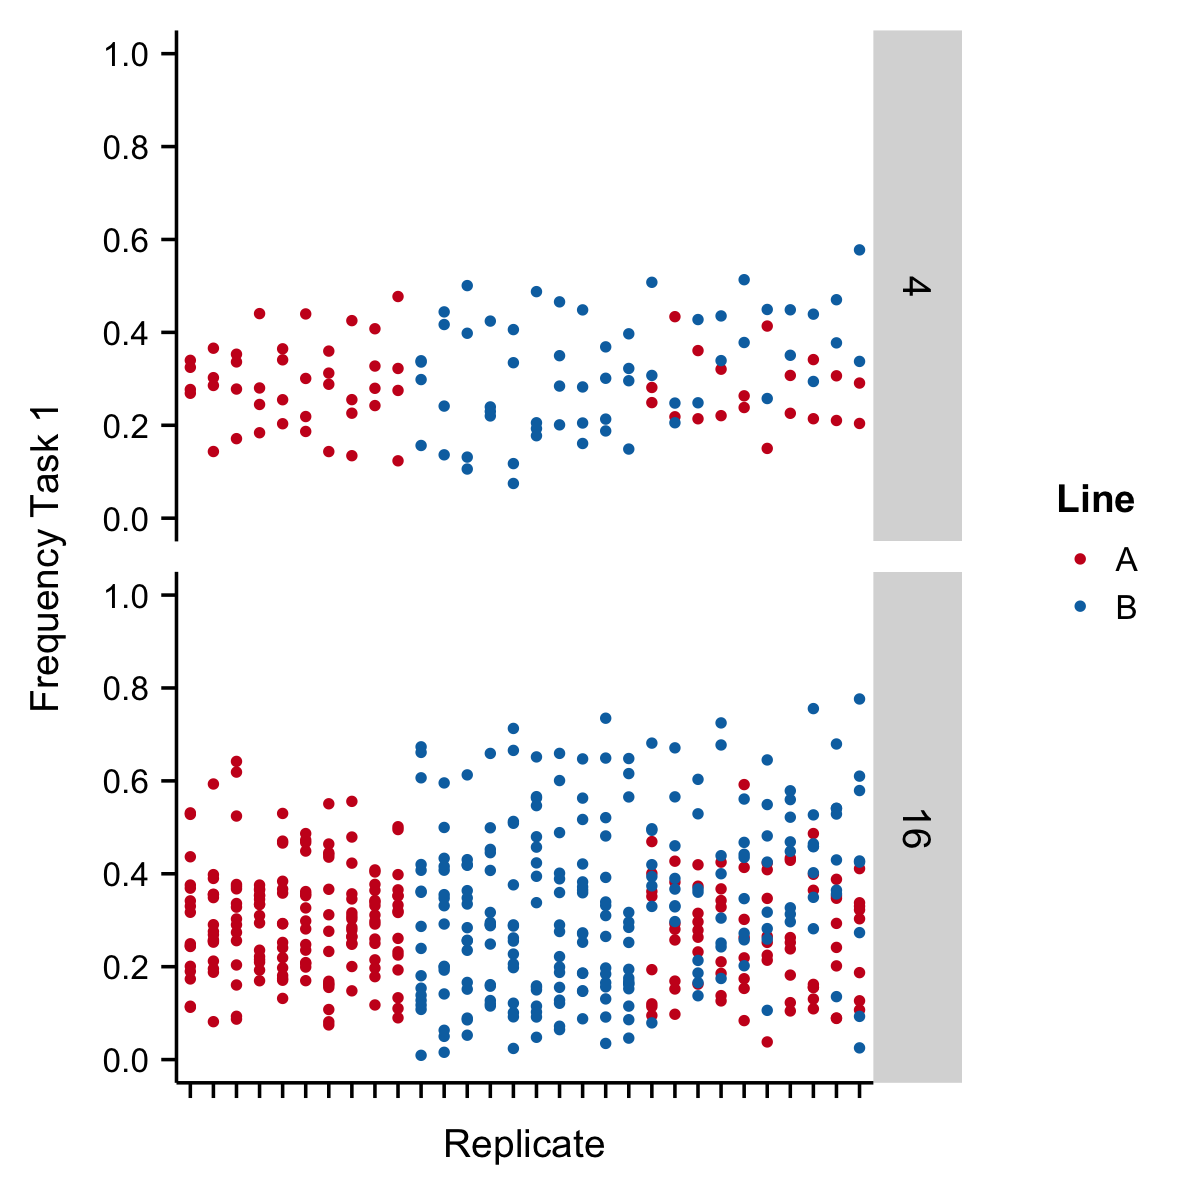
\includegraphics[width=.5\linewidth]{Diff_Etas_HighB.png}
	\caption{Varying threshold stochasticity ($\eta$) by line. The parameter values are identical to those in the base case (Fig.~\ref{fig:base}) with the exception of line-specific threshold slope parameters, $\eta^A = 7, \eta^B = 14$. \\\hspace{0pt}\\
\textbf{Interpretation}: }
	\label{fig:varyetaAB}
\end{figure}

\subsubsection{Varying quit probability $\tau$ by line}

\begin{figure}[H]
	\centering
	\includegraphics[width=.5\linewidth]{{AThreshM_10.00_10.00_AThreshSD_0.10_0.10_BThreshM_10.00_10.00_BThreshSD_0.10_0.10_deltas_0.60_0.60_threshSlope_7_7_Aalpha_2.00_2.00_Balpha_2.00_2.00_quitP_0.20_0.60}.png}
	\caption{Varying quit probability ($\tau$) by line. The parameter values are identical to those in the base case (Fig.~\ref{fig:base}) with the exception of line-specific quit probabilities, $\tau^A = 7, \tau^B = 14$. \\\hspace{0pt}\\
\textbf{Observation}: Higher quit probability ($\tau^B = 0.6$) means that line B ants experience greater turnover rate, which results in smaller variance in frequency of performing task 1.
{\color{blue}
If there is a way to count the number of times the ants ``switch tasks'' (i.e. go to and from the nest), then we could measure a proxy for the average period that the ants spend on one task. The quit probability can be estimated as its inverse.}}
	\label{fig:varytauAB}
\end{figure}

\subsection{\textit{Fixing} across lines and \textit{varying} across tasks}

\subsubsection{Varying task performance efficiency $\alpha$ by task}

\begin{figure}[H]
	\centering
	\includegraphics[width=.5\linewidth]{{New_AThreshM_10.00_10.00_BThreshM_10.00_10.00_deltas_0.60_0.60_threshSlope_7_Aalpha_2.00_6.00_Balpha_2.00_6.00_quitP_0.20}.png}
	\caption{Varying task performance efficiency ($\alpha$) by task. The parameter values are identical to those in the base case (Fig.~\ref{fig:base}) with the exception of task-specific efficiencies, $\alpha_1 = 2, \alpha_2 = 6$. \\\hspace{0pt}\\
\textbf{Observation}: In the single-line cases, the average task 1 performance frequency decreases. This is counterintuitive because I expected that the ants would spend more time performing task 1 because they are less efficient\dots? Also, what is happening in the mixed case?}
	\label{fig:varyalpha12}
\end{figure}

\subsubsection{Varying mean threshold $\mu$ by task}

\begin{figure}[H]
	\centering
	\includegraphics[width=.5\linewidth]{{AThreshM_10.00_20.00_BThreshM_10.00_20.00_deltas_0.60_0.60_threshSlope_7_Aalpha_2.00_2.00_Balpha_2.00_2.00_quitP_0.20}.png}
	\caption{Varying mean threshold ($\mu$) by task. The parameter values are identical to those in the base case (Fig.~\ref{fig:base}) with the exception of task-specific mean thresholds, $\mu_1 = 10, \mu_2 = 20$. \\\hspace{0pt}\\
\textbf{Observation}: No visible change compared to the base case. My intuitive interpretation is that the stimulus for the task with the higher mean threshold (in this case task 2) decreases more slowly, which means that the ants have a smaller probability for performing that task (task 2) but over a longer period of time.}
	\label{fig:varymu12}
\end{figure}


\subsubsection{Varying threshold variance $\sigma$ by task}

\begin{figure}[H]
	\centering
	\includegraphics[width=.5\linewidth]{{AThreshM_10.00_10.00_AThreshSD_0.10_0.30_BThreshM_10.00_10.00_BThreshSD_0.10_0.30_deltas_0.60_0.60_threshSlope_7_7_Aalpha_2.00_2.00_Balpha_2.00_2.00_quitP_0.20_0.20}.png}
	\caption{Varying threshold variance ($\sigma$) by task. The parameter values are identical to those in the base case (Fig.~\ref{fig:base}) with the exception of task-specific threshold variances, $\sigma_1 = 0.1, \sigma_2 = 0.3$. \\\hspace{0pt}\\
\textbf{Observation}: Changing the threshold variance for one task (task 2 in this case) affects the performance frequency of the other task (task 1) as well, as expected. Variance in task 1 performance frequency is greater than in the base case.}
	\label{fig:varysigma12}
\end{figure}


\subsubsection{Varying task demand rate $\delta$ by task}

\begin{figure}[H]
	\centering
	\includegraphics[width=.5\linewidth]{{AThreshM_10.00_10.00_BThreshM_10.00_10.00_deltas_0.60_1.80_threshSlope_7_Aalpha_2.00_2.00_Balpha_2.00_2.00_quitP_0.20}.png}
	\caption{Varying task demand rate ($\delta$) by task. The parameter values are identical to those in the base case (Fig.~\ref{fig:base}) with the exception of task-specific demand rates, $\delta_1 = 0.6, \delta_2 = 1.8$. \\\hspace{0pt}\\
%\textbf{Interpretation}: 
}
	\label{fig:varydelta12}
\end{figure}

\begin{figure}[H]
	\centering
	\includegraphics[width=.5\linewidth]{{AThreshM_10.00_10.00_BThreshM_10.00_10.00_deltas_1.80_1.80_threshSlope_7_Aalpha_2.00_2.00_Balpha_2.00_2.00_quitP_0.20}.png}
	\caption{Higher task demand rate ($\delta$) for both tasks compared to the base case, with $\delta_1 = \delta_2 = 1.8$. \\\hspace{0pt}\\
%\textbf{Interpretation}: 
}
	\label{fig:varydeltaextra}
\end{figure}

\subsection{\textit{Varying} across lines and \textit{Varying} across tasks}

\begin{figure}[H]
	\centering
	\includegraphics[width=.5\linewidth]{{New_AThreshM_10.00_10.00_AThreshSD_0.10_0.10_BThreshM_10.00_10.00_BThreshSD_0.10_0.10_deltas_0.60_0.60_threshSlope_7_7_Aalpha_2.00_6.00_Balpha_6.00_2.00_quitP_0.20_0.20}.png}
	\caption{Varying task efficiency ($\alpha$) by both line and task. The line-and-task-specific efficiencies are $\alpha^A_1 = 2,\ \alpha^A_2 = 6,\ \alpha^B_1 = 6,\ \alpha^B_2 = 6$. \\\hspace{0pt}\\
%\textbf{Interpretation}: 
}
	\label{fig:varyalphaAB12}
\end{figure}

\begin{figure}[H]
	\centering
	\includegraphics[width=.5\linewidth]{{AThreshM_10.00_20.00_BThreshM_20.00_10.00_deltas_0.60_0.60_threshSlope_7_Aalpha_2.00_2.00_Balpha_2.00_2.00_quitP_0.20}.png}
	\caption{Varying mean threshold ($\mu$) by both line and task. The line-and-task-specific efficiencies are $\mu^A_1 = 10,\ \mu^A_2 = 20,\ \mu^B_1 = 20,\ \mu^B_2 = 10$. \\\hspace{0pt}\\
%\textbf{Interpretation}: 
}
	\label{fig:varymuAB12}
\end{figure}

\section{Conclusions so far}

\begin{itemize}
	\item Varying task performance efficiency ($\alpha$) by line
	\begin{itemize}
		\item produces different mean task 1 performance frequencies
		\item produces the `behavioral contagion' pattern
	\end{itemize}
	\item Varying mean threshold ($\mu$) and quit probability ($\tau$) by line
	\begin{itemize}
		\item does NOT produce different mean task 1 performance freq.
		\item produces the `behavioral amplification' pattern
	\end{itemize}
	\item Seems biologically unlikely that the threshold variance ($\sigma$) varies by line

\end{itemize}

\begin{thebibliography}{99}

\bibitem{ulrich2018} Y. Ulrich, J. Saragosti, C. K. Tokita, C. E. Tarnita, D. J. C. Kronauer, ``Fitness benefits and emergent division of labour at the onset of group living,'' \textit{Nature}, vol. 560, pp. 635-638, Aug. 2018.

\end{thebibliography}

\end{document}
%%%%%%%%%%%%%%%%%%%%%%%%%%%

